\section{Evaluation and Analysis}
\label{sec:evaluation}

In the first part of this section, we analyze the well-known benchmark LUBM
and the real-world dataset YAGO and
show cases where these ontologies belong to the parallel tractability classes.
%
In the second part, we evaluate the implementation of Algorithm~$\mathsf{A}_{\text{prc}}$
and compare it to the reasoning system RDFox.
%
In the third part, we examine the effects of the depths of materialization graphs
based on two modified versions of LUBM.



\subsection{Parallel Tractability of the LUBM Datasets and YAGO Ontologies}
\label{sec:lubm-yago}

\textbf{LUBM}. In the Semantic Web community, LUBM
(The Lehigh University Benchmark) is proposed to
facilitate the evaluation of ontology-based systems
in a standard and systematic way.
In the latest version of LUBM,\footnote{http://swat.cse.lehigh.edu/projects/lubm/}
the core ontology contains 48 classes and 32 properties, used to describe the departments and the staff of
universities. By setting a different number of universities for an ontology-generator, users can get datasets of any size based on the core ontology.
%
For the simple form of the core ontology,
the statements about properties, such as inverse property statements,
can be rewritten into datalog rules of the form (R1), (R2) and (R3) in Table~\ref{tab:dhl}.
Most of the statements about classes can be rewritten into datalog rules of the form (T1) and (T3)
in Table~\ref{tab:dhl}. There are six axioms of form (T2) as listed below:
% \begin{enumerate}[leftmargin=8ex,label=($\alpha_{\arabic*}$),ref=$\alpha_{\arabic*}$]
%   \item $\texttt{Person}\sqcap\texttt{CourseTaker}\sqsubseteq\texttt{Student}$\label{lubm:a1}
%   \item $\texttt{Person}\sqcap\texttt{OrganizationWorker}\sqsubseteq\texttt{Employee}$\label{lubm:a2}
%   \item $\texttt{Person}\sqcap\texttt{DepartmentHead}\sqsubseteq\texttt{Chair}$\label{lubm:a3}
%   \item $\texttt{Person}\sqcap\texttt{ProgramHead}\sqsubseteq\texttt{Director}$\label{lubm:a4}
%   \item $\texttt{Person}\sqcap\texttt{CourseAssistant}\sqsubseteq\texttt{TeachingAssistant}$\label{lubm:a5}
%   \item $\texttt{Person}\sqcap\texttt{CollegeHead}\sqsubseteq\texttt{Dean}$\label{lubm:a6}
% \end{enumerate}
\begin{align}
\texttt{Person}\sqcap\texttt{CourseTaker} & \sqsubseteq\texttt{Student}\label{lubm:a1}\tag{$\alpha_1$}\\
\texttt{Person}\sqcap\texttt{OrganizationWorker} & \sqsubseteq\texttt{Employee}\label{lubm:a2}\tag{$\alpha_2$}\\
\texttt{Person}\sqcap\texttt{DepartmentHead} & \sqsubseteq\texttt{Chair}\label{lubm:a3}\tag{$\alpha_3$}\\
\texttt{Person}\sqcap\texttt{ProgramHead} & \sqsubseteq\texttt{Director}\label{lubm:a4}\tag{$\alpha_4$}\\
\texttt{Person}\sqcap\texttt{CourseAssistant} & \sqsubseteq\texttt{TeachingAssistant}\label{lubm:a5}\tag{$\alpha_5$}\\
\texttt{Person}\sqcap\texttt{CollegeHead} & \sqsubseteq\texttt{Dean}\label{lubm:a6}\tag{$\alpha_6$}
\end{align}
In the above axioms, the six concepts \texttt{CourseTaker}, \texttt{OrganizationWorker},
\texttt{DepartmentHead}, \texttt{ProgramHead}, \texttt{CourseAssistant}
and \texttt{CollegeHead} have corresponding definitions.
For example, the concept \texttt{CourseTaker} is defined by:
\begin{align}
  \texttt{CourseTaker} & \equiv\exists\texttt{take}.\texttt{Course},\notag\\
  \intertext{which is equivalent to the two axioms of simple form,}
  \exists\texttt{take}.\texttt{Course} &
                                         \sqsubseteq\texttt{CourseTaker} \mbox{ and}\label{coursetaker1}\\
  \texttt{CourseTaker} &
                         \sqsubseteq\exists\texttt{take}.\texttt{Course}.\label{coursetaker2}
\end{align}
Axiom~\eqref{coursetaker1} corresponds to form
(T3). Axiom~\eqref{coursetaker2} requires existentially quantified
variables in the rule head when rewriting the axiom into a logic rule:
\begin{align}
\texttt{CourseTaker}(x)\rightarrow\exists y(\texttt{take}(x,y)\wedge
  \texttt{Course}(y))\label{tau}\tag{$\tau$}
\end{align}
where a free variable $y$ is introduced. This kind of axiom is a general case of (T4) in Table~\ref{tab:dhl}
for which $A$ is actually replaced by the top concept $\top$.
Similarly to how we handle (T4), we can also eliminate the free variable $y$
in Rule~\eqref{tau} via Skolemization, i.e., by replacing the variable $y$ with a new constant $o$.
In this way, Rule~\eqref{tau} can be rewritten into $\texttt{CourseTaker}(x)\rightarrow\texttt{take}(x,o)\wedge \texttt{Course}(o)$.
If we only focus on the materialization task, the rewriting approach via Skolemization guarantees
correctness \cite{GrauHKKMMW13}.
On the other hand, Rule~\eqref{tau} is not considered when using OWL RL reasoners to handle LUBM \cite{UrbaniKMHB12,WeaverH09}.
In summary, if the rewriting approach is used for the above kind of rule,
the core ontology can be expressed in DHL.
We can further check that the concepts occurring in (\ref{lubm:a1}--\ref{lubm:a6})
are all simple concepts. Thus,
the materialization of LUBM datasets is tractable in parallel and can be handled by
Algorithm~$\mathsf{A}_{\text{prc}}$.


\textbf{YAGO}. The knowledge base YAGO\footnote{http://www.mpi-inf.mpg.de/home/}
is constructed from Wikipedia and WordNet. The latest version
YAGO3 \cite{MahdisoltaniBS15} has millions of facts.
In order to balance the expressiveness and computing efficiency,
a YAGO-style language, called the \emph{YAGO model}, is proposed based on
a slight extension of RDFS \cite{SuchanekKW08}. The YAGO model defines
a set of properties: \texttt{domain, range, subClassOf, subRelationOf} and \texttt{type},
and a set of classes: \texttt{entity, class, relation} and \texttt{acyclicTransitiveRelation}.
The facts in the YAGO model are stated by triples, e.g., $(r_1,
\texttt{subRelationOf}, r_2)$,
which are similar to RDFS statements.
A group of rules for reasoning over YAGO ontologies
is specified by \citet{SuchanekKW08}:
\begin{align}
(r,\texttt{domain}, c), (x, r, y) & \rightarrow (x,
    \texttt{type}, c)\label{yago:r1}\\
(r,\texttt{range}, c), (x, r, y) & \rightarrow (y,
    \texttt{type}, c)\label{yago:r2}\\
(c_1, \texttt{subClassOf}, c_2), (x, \texttt{type}, c_1)
    & \rightarrow (x, \texttt{type}, c_2)\label{yago:r3}\\
(r_1, \texttt{subRelationOf}, r_2), (x, r_1, y) & \rightarrow
    (x, r_2, y)\label{yago:r4}\\
(r, \texttt{type}, \texttt{acyclicTransitiveRelation}), (x,
    r, y), (y, r, z) & \rightarrow (x, r, z)\label{yago:r5}
\end{align}
According to the semantics given to YAGO \cite{SuchanekKW08}, the built-in properties in YAGO,
i.e., \texttt{domain, range, subClassOf, subRelationOf} and \texttt{type} act in the same
way as the terms in RDFS statements of the form (S1--S5) in Table~\ref{tab:rdfs}, respectively.
In contrast to RDFS, YAGO also allows for defining
transitive properties using the
class \texttt{acyclicTransitiveRelation}; further, any fact in some YAGO ontology cannot be
described using blank nodes. By carefully checking the rules (\ref{yago:r1}--\ref{yago:r5}) for reasoning over YAGO ontologies,
one can see that these rules can be rewritten into datalog rules
of the form (T3),\footnote{Both of Rule (\ref{yago:r1}) and
Rule (\ref{yago:r2}) can be rewritten into (T3).} (T1), (R1) and (R3) in Table~\ref{tab:dhl}, respectively.
Based on the above analysis, any YAGO ontology can be expressed in DHL
and satisfies the simple-concept and the simple-role restrictions. We then have that,
for any well-constructed class of YAGO ontologies,
Algorithm~$\mathsf{A}_{\text{prc}}$
can handle all of the ontologies in the class.

In addition to LUBM and YAGO, we further investigate different kinds of ontologies and datasets
including benchmarks, real-world ontologies and datasets that can be
expressed in ontology languages.
These ontologies and datasets are collected from the Prot\'{e}g\'{e}
ontology
library,\footnote{http://protegewiki.stanford.edu/wiki/Protege\textunderscore
  Ontology\textunderscore Library}
Swoogle\footnote{http://swoogle.umbc.edu/} and the Oxford ontology library.\footnote{http://www.cs.ox.ac.uk/isg/ontologies/lib/}
Based on the analysis of these ontologies, we found that, ignoring imports, many of them
belong to $\mathcal{D}_{\textit{\text{dhl}}}$ or $\mathcal{D}_{\textit{\text{dhl}}(\circ)}$.
All of these investigated ontologies and the analysis results are available online.\footnote{https://github.com/quanzz/PT}

\begin{table}
\centering
\caption{The statistics of the test ontologies, where $\sharp$concept
  denotes the number of concept names, $\sharp$role the number of role
  names, $\sharp$axiom the number of TBox and RBox axioms,
  $\sharp$individual  the number of individuals and $\sharp$assertion
  the number of assertions in the ontology}
\begin{tabular}{|l|r|r|r|r|r|}
\hline
ontology&$\sharp$concept&$\sharp$role&$\sharp$axiom&$\sharp$individual&$\sharp$assertion\\
\hline
lubm-50&\multirow{5}{*}{48}&\multirow{5}{*}{32}&\multirow{5}{*}{99}&1,082,818&11,601,923\\
lubm-100&&&&2,179,766&23,837,579\\
lubm-150&&&&3,243,523&35,466,709\\
lubm-200&&&&4,341,309&46,537,764\\
lubm-250&&&&5,421,894&58,125,155\\
\hline
yago-core&65,318&74&55,615&4,077,882&45,277,896\\
\hline
\end{tabular}
\label{tab:onto}
\end{table}

\begin{table}
\centering
\caption{The reasoning time results in seconds}
{\setlength{\tabcolsep}{1.5mm}
\begin{tabular}{|l|r|r|r|r|r|r|r|}
\hline
&\small$\sharp$thread&lubm-50&lubm-100&lubm-150&lubm-200&lubm-250&yago-core\\
\hline
\multirow{5}{*}{ \small{\textbf{ParallelDHL}}}&1&93.66&213.75&376.39&498.34&693.49&773.06\\
                    &4&21.71&54.03&111.2&123.76&159.82&223.4\\
                    &8&9.44&23.04&55.78&67.29&86.41&98.33\\
                    &16&4.02&12.7&20.9&35.63&43.91&47.08\\
                    &24&4.06&9.82&16.84&22.31&27.47&34.48\\
\hline
\multirow{5}{*}{ \small{\textbf{RDFox}}}&1&23.01&42.8&71.92&88.64&111.96&105.73\\
                    &4&5.97&11.64&18.5&22.31&25.59&35.5\\
                    &8&4.88&5.89&9.95&11.21&12.8&19.07\\
                    &16&3.18&3.75&8.37&9.16&12.19&13.22\\
                    &24&1.92&3.9&6.21&7.74&9.58&11.81\\
\hline
\end{tabular}}
\label{tab:result}
\end{table}


\subsection{Evaluating the Implementation of Algorithm~$\mathsf{A}_{\text{prc}}$}

We implement a prototype system ParallelDHL for DHL$(\circ)$ materialization
based on Algorithm~$\mathsf{A}_{\text{prc}}$. Since ParallelDHL is
evaluated on a
platform which has limited memory space and a fixed number of processors,
the parallel assumption given in Section~\ref{sec:alg-bsc} does not apply to ParallelDHL.
In the implementation of ParallelDHL, we use a hash function to map any rule instance
to the identifier of some processor. Thus, when performing ParallelDHL,
each processor handles a group of rule instances.

We run ParallelDHL on LUBM and YAGO to further analyze these
two kinds of ontologies. We also use the reasoning system RDFox \cite{MotikNPHO14}
for comparison. We use five generated LUBM datasets, lubm-50, lubm-100, lubm-150, lubm-200
and lubm-250, where lubm-50 contains the descriptions of 50
universities (and analogously for the other datasets). For YAGO, we use its core version, denoted by yago-core.\footnote{
The yago-core ontology is available at https://www.mpi-inf.mpg.de/departments/databases-and-information-systems/research/yago-naga/yago/downloads/.}
The yago-core ontology is a subset of the full YAGO dataset without any imports.
It does not include datatype statements, the links
between different data sources, the degrees of confidence and other kinds of
annotations that we do not consider in this work. The statistics of the above ontologies is given in Table~\ref{tab:onto}.
The running platform for this experiment is a server with 50 Gigabyte RAM and eight physical cores, in each core
three logical threads can be allocated.

We materialize the LUBM datasets and the yago-core ontology with ParallelDHL and RDFox using different numbers of
threads (1, 4, 8, 16 and 24, respectively).
The reasoning times are given in Table~\ref{tab:result}. We also give Figure~\ref{fig:reasoningtime} to
graphically compare the two systems.
In Figure~\ref{fig:reasoningtime}(left), the abscissa records the five
LUBM datasets and
the ordinate records the reasoning times in seconds with $24$ threads being allocated.
In Figure~\ref{fig:reasoningtime}(right), the abscissa records the numbers of threads and
the ordinate records the reasoning times in seconds over the yago-core ontology.


\begin{figure}[htbp]
\begin{center}
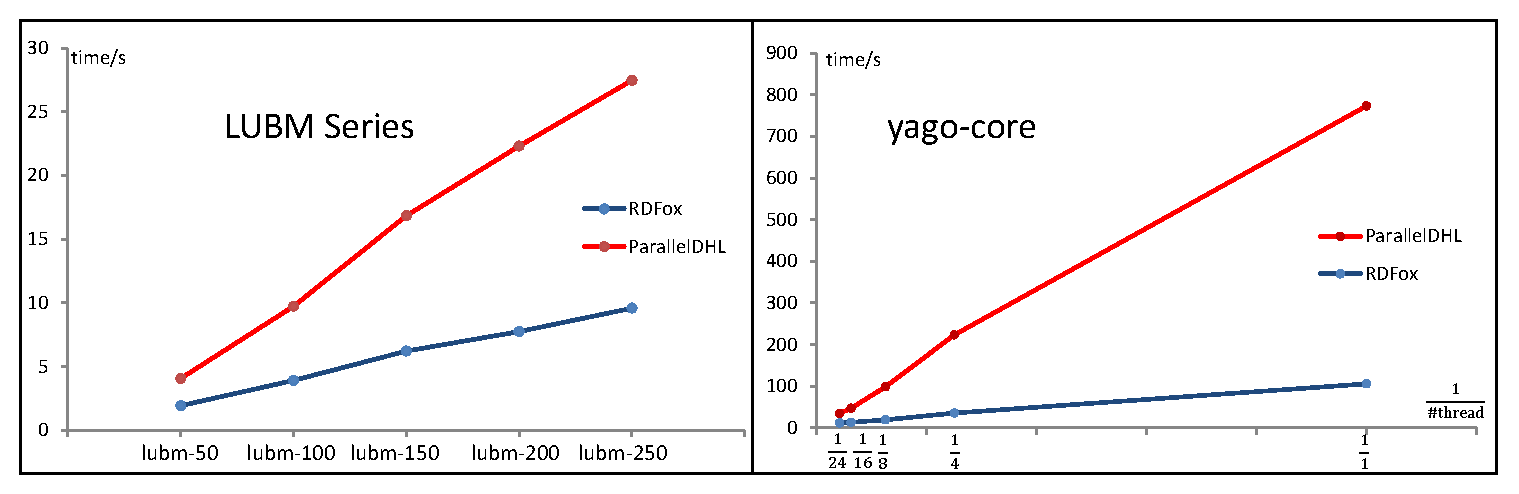
\includegraphics[width=\textwidth]{fig-reasoningtime.eps}
\caption{(left) The reasoning times over the LUBM ontologies; (right)
  the reasoning times over yago-core}
\label{fig:reasoningtime}
\end{center}
\end{figure}

From Table~\ref{tab:result}, we can see that for lubm-50 the two systems perform similarly.
For the other ontologies, ParallelDHL scales comparable to RDFox with several threads being allocated.
For lubm-250 and yago-core, when only one thread is used, ParallelDHL
is significantly slower.
The reason is that the computation of the relation $S_{\textit{\!\tiny rch}}$ requires a large amount of time. When
four and more threads are allocated, ParallelDHL has a better efficiency.
Although ParallelDHL is by far not as optimized as RDFox, it also shows the scalability.
For both of RDFox and ParallelDHL,
we can see a linear trend of the reasoning times
in Figure~\ref{fig:reasoningtime}(left) and
an obvious downtrend of the reasoning times with an increasing number of threads
in Figure~\ref{fig:reasoningtime}(right).
This also indicates that ParallelDHL will finish the materialization tasks on the test ontologies
in a shorter period of time with more threads being allocated.

\subsection{Depths of Materialization Graphs}

From the complexity analysis for Algorithm~$\mathsf{A}_{\text{bsc}}$ (see Section~\ref{sec:alg-bsc}),
we have that the computing time of
Algorithm~$\mathsf{A}_{\text{bsc}}$ depends on the sizes of the input ontologies and the
numbers of iterations of \ref{alg1:updateG},
which is equal to the \emph{depth of the target materialization
  graph}, which we abbreviate with \emph{MG-depth} in the remainder.
Thus, the MG-depth also determines the computing time of
Algorithm~$\mathsf{A}_{\text{bsc}}$ in theory.
This conclusion also applies to Algorithm~$\mathsf{A}_{\text{opt}}$ and Algorithm~$\mathsf{A}_{\text{prc}}$
based on the analysis in Section~\ref{sec:opt} and Section~\ref{sec:practicalAlg}, respectively.
In this part, we examine the effects of MG-depths.

\begin{figure}[htbp]
\begin{center}
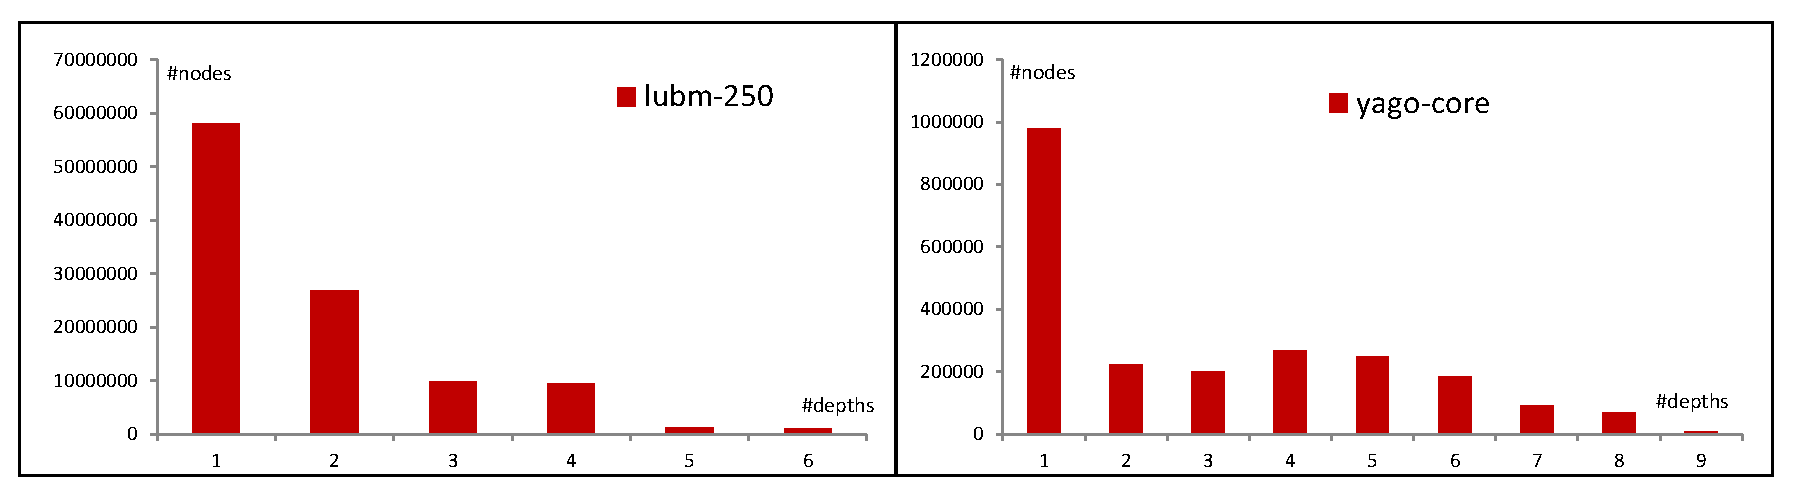
\includegraphics[width=1\textwidth]{fig-graphdepth.eps}
\caption{The numbers of nodes in different depths of lubm-250 (left)
  and yago-core (right)}
\label{fig:graphdepth}
\end{center}
\end{figure}

\textbf{MG-Depths of LUBM and YAGO.}
For the five generated LUBM datasets and the yago-core ontology, we record the MG-depth
for each ontology and the number of nodes in different depths.
We have that all of the LUBM datasets have an MG-depth of 6,
and the MG-depth of the yago-core ontology is 9.
The two histograms in Figure~\ref{fig:graphdepth} visualize the number
of nodes in different depths for lubm-250 and yago-core,
respectively.
The abscissa records the depths from the bottom of a materialization
graph to the top with
the histograms showing the amount of nodes for each depth.
%
From the above results, we can see that the MG-depths are far less than
the sizes of the input ontologies. In these cases, the input ontology size
turns out to be the dominant factor for the reasoning efficiency.
This is also shown in Figure~\ref{fig:reasoningtime}(left) for the LUBM datasets,
where the reasoning times grow proportionally with the increasing number
of universities.
%
Thus, the above experiments hardly show the effects of MG-depths.

\begin{table}
\centering
\caption{The statistics of the generated datasets}
\begin{tabular}{|l|r|r|r|r|r|r|}
\hline
ontology&$\sharp$concept&$\sharp$role&$\sharp$axiom&$\sharp$individual&$\sharp$assertion&MG-depth\\
\hline
ptu-$4m$-1&\multirow{10}{*}{51}&\multirow{10}{*}{34}&\multirow{10}{*}{102}&\multirow{10}{*}{4,000,440}&8,000,839&8,000,799\\
ptu-$4m$-2&&&&&8,000,837&4,000,399\\
ptu-$4m$-4&&&&&8,000,835&2,000,199\\
ptu-$4m$-8&&&&&8,000,833&1,000,099\\
ptu-$4m$-16&&&&&8,000,831&500,049\\
nptu-$4m$-1&&&&&8,000,839&8,000,799\\
nptu-$4m$-2&&&&&8,000,837&4,000,399\\
nptu-$4m$-4&&&&&8,000,835&2,000,199\\
nptu-$4m$-8&&&&&8,000,833&1,000,099\\
nptu-$4m$-16&&&&&8,000,831&500,049\\
\hline
\end{tabular}
\label{tab:generated}
\end{table}

\textbf{Generating Ontologies of Different MG-Depths}.
In order to examine the effects of MG-depths, we consider modifying the core LUBM ontology
such that ontologies of different MG-depths can be obtained.
Inspired by Example~\ref{exp:simpleC},
we add to the core LUBM ontology the following three axioms to
describe the reference relationships among articles:
\begin{align}
\exists\texttt{referTo}.\texttt{CollegeArticle} & \sqsubseteq\texttt{CollegeConference}\label{ptu:a1}\tag{$\beta_1$}\\
\exists\texttt{cite}.\top & \sqsubseteq\texttt{CollegeSession}\label{ptu:a2}\tag{$\beta_2$}\\
\texttt{CollegeConference}\sqcap\texttt{CollegeSession} & \sqsubseteq\texttt{CollegeArticle}\label{ptu:a3}\tag{$\beta_3$}
\end{align}
where Axiom~\eqref{ptu:a1} states that any article referring to a
college article is published in a college conference,
Axiom~\eqref{ptu:a2} defines that any article having citations is
published in a college session and Axiom~\eqref{ptu:a3} states that
any article published in both a college conference and a college
session is a college article.

We name the above new ontology PTU.
Based on the newly added axioms in PTU, we further modify the ontology-generator
of LUBM such that a \emph{reference chain} of articles can be generated as follows:
$\texttt{referTo}(\texttt{a}_i,\texttt{a}_{i+1})$ and
$\texttt{cite}(\texttt{a}_i,\texttt{a}_{i+1})$ ($i\in\{0,1,2,...\}$),
where $\texttt{a}_i$ denotes an article instance.
As discussed in Section~\ref{sec:lubm-yago},
the original core ontology of LUBM is tractable in parallel via
Skolemization. Further, it can be checked that the concepts in PTU
are all simple concepts. Thus, PTU belongs to the parallel tractability class.
For comparison, we create another core ontology, named NPTU, which
is not tractable in parallel. NPTU is almost the same as PTU except that
Axiom~\eqref{ptu:a2} in PTU is replaced by:
\begin{align}
\exists\texttt{cite}.\texttt{CollegeArticle}\sqsubseteq\texttt{CollegeSession}\label{nptu:a1}\tag{$\beta_4$}
\end{align}
which describes that any article citing a college article is published in a
college session.
It can be checked that NPTU does not satisfy the simple-concept
restriction following analogous arguments to those given in Example~\ref{exp:dhl}.

The two core ontologies, PTU and NPTU,
and the modified ontology-generator are available online.\footnote{https://github.com/quanzz/PT}
To reduce the effects of ontology sizes, we generate five datasets of
the similar sizes for PTU (NPTU, respectively), denoted by
ptu-$4m$-$i$ (nptu-$4m$-$i$, respectively), $i\in\{1,2,4,8,16\}$,
where $i$ is the number of article reference chains
and $4m$ denotes that $4$ million articles are involved on average in all of the reference chains.
The statistics for the generated datasets are given in Table~\ref{tab:generated}.
Table~\ref{tab:generated} shows that the datasets ptu-$4m$-$i$ ($i\in\{1,2,4,8,16\}$)
have an almost identical number of assertions while the MG-depth
decreases proportionally, e.g., the MG-depth of ptu-$4m$-$1$ is
$8,000,799$, while the MG-depth of ptu-$4m$-$16$ is just
$500,049$. This is
analogous for the datasets nptu-$4m$-$i$ ($i\in\{1,2,4,8,16\}$).


\textbf{Experimental Results and Analysis}.
Table~\ref{tab:speedup} compares the reasoning times and
speedups\footnote{The speedup is computed by $\frac{T_1}{T_n}$ where $T_1$ is the computing time
using 1 thread and $T_n$ is the computing time using $n$ thread(s).}
of ParallelDHL and RDFox for materializing ptu-$4m$-1 and
nptu-$4m$-1.\footnote{The detailed experimental results are available
  online at https://github.com/quanzz/PT.}
Figure~\ref{fig:diffdepths} and~\ref{fig:diffthreads} show the trends of
reasoning times. Specifically, the two line graphs of Figure~\ref{fig:diffdepths}
show the reasoning times in seconds of ParallelDHL and RDFox over
all the generated datasets with 24 threads being allocated. In Figure~\ref{fig:diffthreads},
the abscissas of the two line graphs record the numbers of threads and
the ordinates record the reasoning times over ptu-$4m$-1 and nptu-$4m$-1, respectively.

\begin{figure}[htbp]
\begin{center}
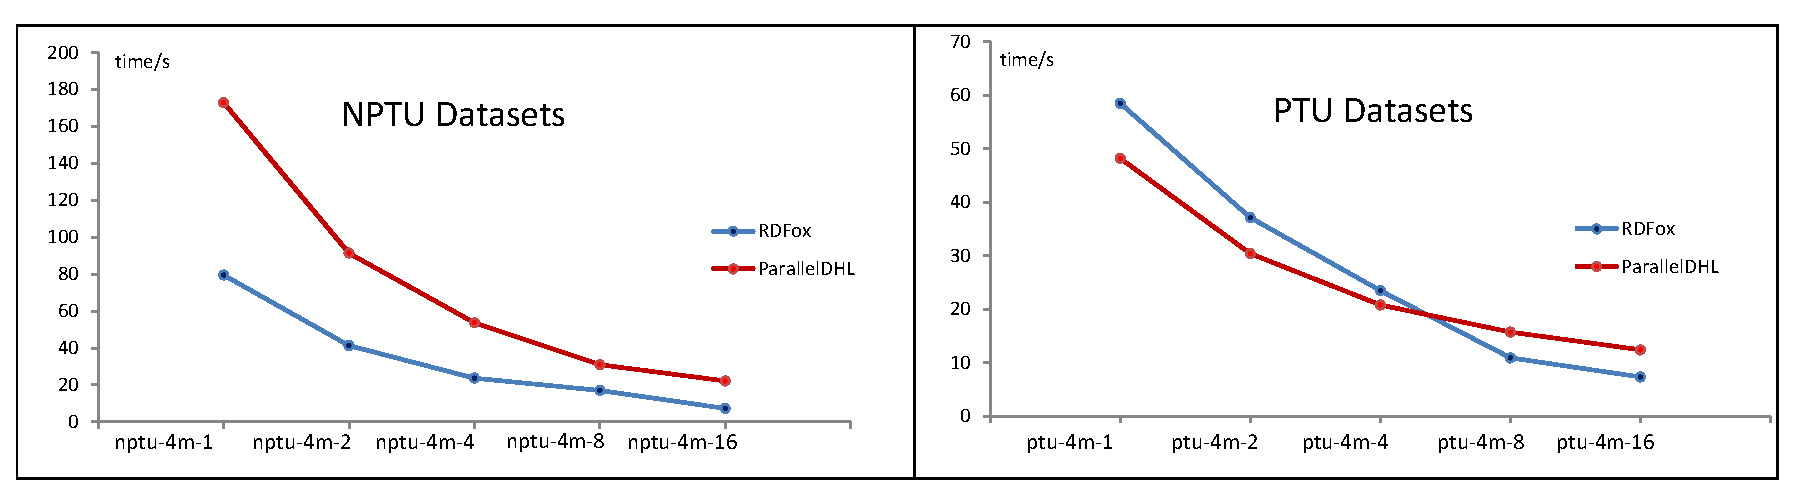
\includegraphics[width=1\textwidth]{fig-diff-depths.eps}
\caption{(left) reasoning times over the PTU datasets; (right)
  reasoning times over the NPTU datasets}
\label{fig:diffdepths}
\end{center}
\end{figure}

Figure~\ref{fig:diffdepths} shows that MG-depths indeed determines
the reasoning times.
For the five datasets ptu-$4m$-$i$, $i\in\{1,2,4,8,16\}$, the experimental
results show an obvious downtrend of the reasoning times with declining MG-depths for
both ParallelDHL and RDFox (see Figure~\ref{fig:diffdepths}(left)).
The downtrend of reasoning times also exists
when handling the datasets nptu-$4m$-$i$, $i\in\{1,2,4,8,16\}$ (see Figure~\ref{fig:diffdepths}(right)).
Although the PTU and NPTU datasets are unrealistic in practice, these experiments indeed
verify that MG-depths determines the reasoning time in parallel
considering that the input ontology sizes are close.

\begin{table}
\centering
\caption{The reasoning-times in seconds and speedups}
% \begin{tabular}{|l|r|r|r|r|r|}
% \hline
% &\small$\sharp$thread&nptu-$4m$-1&speedup&ptu-$4m$-1&speedup\\
% \hline
% \multirow{5}{*}{ \small{\textbf{ParallelDHL}}}&1&135.79&1&252.13&1\\
%                                 &4&142.34&0.95&147.20&1.71\\
%                                 &8&145.04&0.93&102.83&2.45\\
%                                 &16&156.05&0.87&56.48&4.46\\
%                                 &24&172.81&078\BG{decimal point missing?}&48.19&5.23\\
% \hline
% \multirow{5}{*}{ \textbf{RDFox}}&1&50.95&1&20.55&1\\
%                                 &4&72.42&0.7&56.48&0.36\\
%                                 &8&74.43&0.68&54.52&0.38\\
%                                 &16&74.23&0.69&60.98&0.34\\
%                                 &24&79.46&0.64&58.47&0.35\\
% \hline
% \end{tabular}
\begin{tabular}{|l|r|r|r|r|r|}
\hline
&\small$\sharp$thread&ptu-$4m$-1&speedup&nptu-$4m$-1&speedup\\
\hline
\multirow{5}{*}{ \small{\textbf{ParallelDHL}}}&1&252.13&1&135.79&1\\
                                &4&147.20&1.71&142.34&0.95\\
                                &8&102.83&2.45&145.04&0.93\\
                                &16&56.48&4.46&156.05&0.87\\
                                &24&48.19&5.23&172.81&0.78\\
\hline
\multirow{5}{*}{ \textbf{RDFox}}&1&20.55&1&50.95&1\\
                                &4&56.48&0.36&72.42&0.7\\
                                &8&54.52&0.38&74.43&0.68\\
                                &16&60.98&0.34&74.23&0.69\\
                                &24&58.47&0.35&79.46&0.64\\
\hline
\end{tabular}
\label{tab:speedup}
\end{table}

We now discuss the issue of parallel tractability based on the experimental
results of ptu-$4m$-1 and nptu-$4m$-1.
For the dataset ptu-$4m$-1, the trends of reasoning times are different
between ParallelDHL and RDFox.
It can be checked from Table~\ref{tab:speedup} that
RDFox does not benefit from the allocation of several threads for ptu-$4m$-1;
the speedups under different numbers of threads stay around 1.
This means that reasoning times are not reduced with an increasing number of threads.
ParallelDHL shows a better speedup effect. With only one allocated thread, ParallelDHL finishes
the materialization of ptu-$4m$-1 in $135.79$ seconds (Table~\ref{tab:speedup}). When four and more threads
are allocated, the reasoning performance is improved significantly.
The maximal speedup is $5.23$ using $24$ threads.
Specially, with $16$ or more threads, ParallelDHL
requires less time to finish the materialization compared to RDFox.
From Figure~\ref{fig:diffthreads}(left), there is an obvious downtrend of the reasoning times
from one thread to $24$ threads.
The main reason for the difference between ParallelDHL and RDFox
is that the PTU ontology is tractable in parallel and ParallelDHL
is optimized based on SWD paths. The PTU ontology follows the
simple-concept restriction. Thus, there is no twisting path in
the materialization graph of ptu-$4m$-1 although all articles are involved
in one reference chain. This allows for computing the relation $S_{\textit{\!\tiny
    rch}}$ only once in the second iteration of \ref{alg3:updateG} of Algorithm~$\mathsf{A}_{\text{prc}}$
when handling ptu-$4m$-1 (referring to the analysis for Example~\ref{exp:simpleC}).
It can also be checked that all the axioms of the form \texttt{CollegeArticle}$(a_i)$ occur in
an SWD path. Thus, the optimization based on SWD paths works when handling ptu-$4m$-1.
For RDFox, since it is not optimized specially for this case, it performs the task of
materialization over ptu-$4m$-1 similarly to that over nptu-$4m$-1;
specifically, the axioms of the form \texttt{CollegeArticle}$(a_i)$ are derived sequentially.
From Figure~\ref{fig:diffdepths}(left), we can see that the optimization used in ParallelDHL
also leads to a better performance compared to
RDFox when handling ptu-$4m$-1, ptu-$4m$-2 and ptu-$4m$-4 using $24$ threads.

\begin{figure}[htbp]
\begin{center}
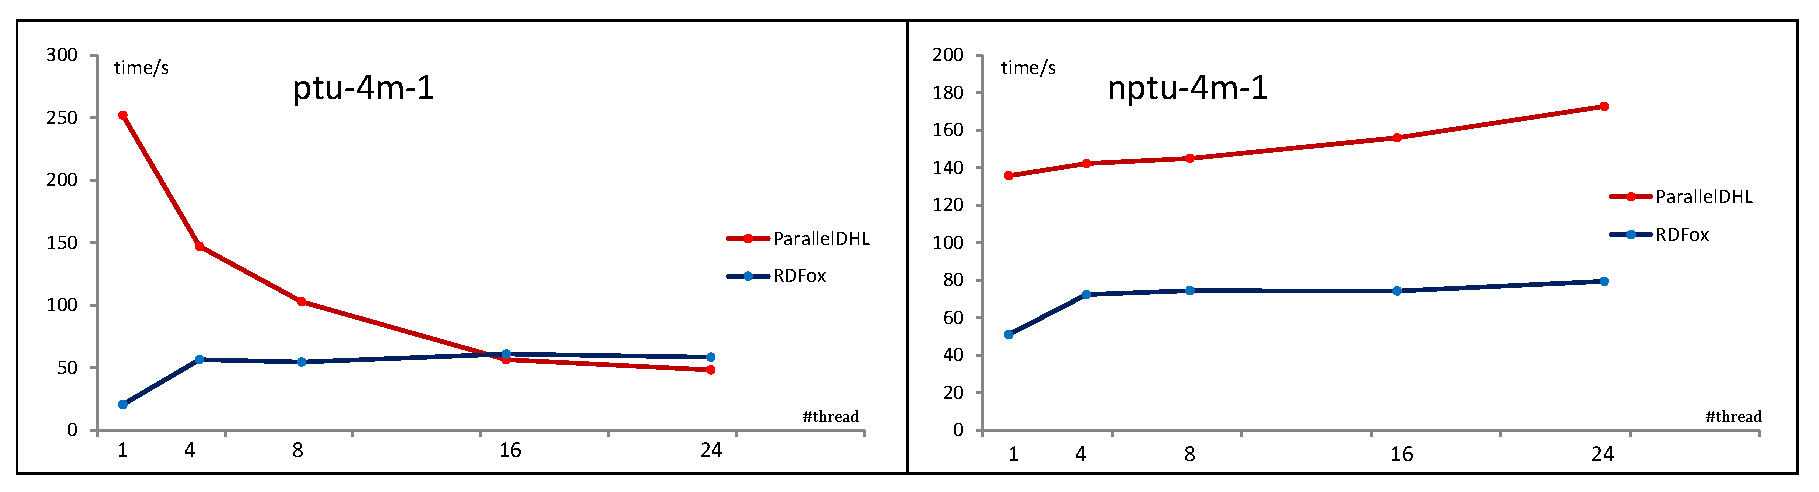
\includegraphics[width=1\textwidth]{fig-diff-threads.eps}
\caption{(left) the reasoning times over nptu-$4m$-1; (right) the reasoning times over ptu-$4m$-1.}
\label{fig:diffthreads}
\end{center}
\end{figure}

From Figure~\ref{fig:diffthreads}(right),
we can see that for both ParallelDHL and RDFox the reasoning efficiency is not
improved when several threads are allocated. On the contrary, with less than 24 threads allocated,
materialization takes less time. In detail,
the reasoning time of RDFox using $24$ threads
is $79.46$ seconds, while it is $50.95$ seconds using only one thread.
Further, the speedups of RDFox stay below $1$ using more than $1$ threads (see Table~\ref{tab:speedup}).
This means that the reasoning times cannot be reduced with several threads being
allocated.
This maybe unexpected behavior is also shown by ParallelDHL and is caused by the issue of path twisting.
The NPTU ontology does not follow the simple-concept restriction since
the concepts \texttt{CollegeConference} and \texttt{CollegeSession} are not simple.
The materialization of nptu-$4m$-$i$ ($i\in\{1,2,4,8,16\}$) suffers from the issue
of path twisting which is similar to the case in Example~\ref{exp:dhl}.
Specifically, the axioms of the form \texttt{CollegeArticle}$(a_i)$ are
the joint nodes in the twisted path.
According to the analysis in Example~\ref{exp:dhl}, parallel computation can hardly
handle this case. Moreover, the dataset nptu-$4m$-1 has only one
article reference chain. This means that all
the axioms of the form \texttt{CollegeArticle}$(a_i)$ actually
appear in one path of the target materialization graph.
Thus, they depend on each other and cannot be derived in parallel.
On the other hand, the working mechanism of ParallelDHL and RDFox is based on
a thread pool, where several threads are maintained and scheduled.
The maintenance and scheduling of the thread pool also produces
overheads, in particular, when the parallel computation
cannot improve the total efficiency.
This is why the materialization of nptu-$4m$-1 using $1$
thread has a better performance.


%%% Local Variables:
%%% mode: latex
%%% TeX-master: "parallel-tractability-J"
%%% End:
